\section{Kommunikationsenhet}
Kommunikationsenheten ansvarar för att förmedla information mellan de olika enheterna i systemet. 
Kommunikationen mellan PC och roboten kommer att ske via blåtand. Kommunikation mellan de olika delsystemen på roboten kommer att ske med en så kallad SPI-buss.

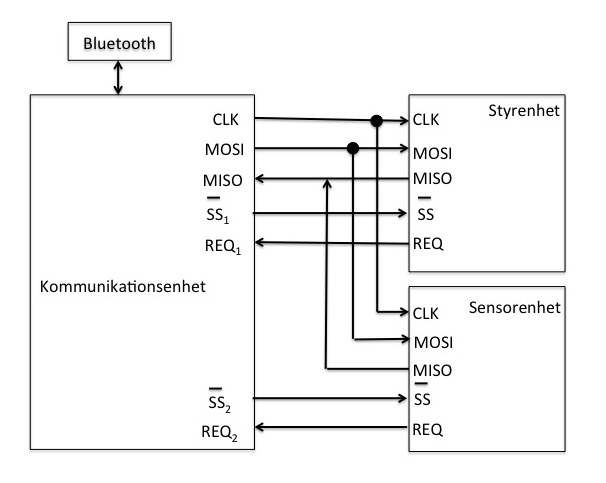
\includegraphics[angle=0,scale=0.5]{bilder/SPI-buss.png}

\subsection{Blåtand}
Kommunikationsenheten kommer ha en blåtandsmodul av typ Firefly, ansluten via
UART, för att kommunicera med mjukvaran på PCn.

En blinkande röd LED på blåtandsenheten visar att enheten är redo för en
blåtandsanslutning medan en stadigt grön LED indikerar att blåtandsenheten har
en aktiv anslutning.

\subsubsection{Överföringar}
Blåtandsenheten kommer skicka och ta emot information från PCn enligt formatet
8N1, det vill säga vi skickar data i enheter om 8 bitar (en byte), använder oss
inte av någon paritetsbit, har en bit som slutbit och en bit som startbit
(som inte anges). Totalt kommer alltså 10 bitar skickas för att överföra 8
bitar.

Kommunikationsenheten agerar master för SPI-bussen och tar därför emot all data
som skickas mellan systemets olika moduler. För att skicka rätt data till rätt
mottagare så utnyttjar kommunikationsenheten addressfältet i meddelandets
header.

\subsection{SPI}
\label{sec:SPI}
SPI bussen är ett kommunikationssystem som använder ett så kallat Master-Slav system. I roboten kommer kommunikationsenheten att vara Master. Systemet kommer att ha två slavar i form av styrenheten och sensorenheten.
Detta betyder att all kommunikation kommer att behöva gå via kommunikationsenheten. SPI bussen arbetar alltid i så kallat full duplex läge vilket betyder att överföringar kan ske i två riktningar samtidigt. Således kan 2 bits skickas via SPI bussen på 1 klockcykel. 

Robotens kommunikationssystem kommer att fungera så att styr- och sensorenheten har möjlighet att ta initiativ till överföringar till och från kommunikationsenheten. Detta är inte standard på SPI-bussen utan löses med två stycken extrasignaler vi kommer att kalla för REQ-signaler. Alla sorters kommunikation kommer att styras med hjälp av avbrott, som är ett utmärkt sätt att hantera plötsliga externa kommandon. REQ signalen kommer att generera ett avbrott hos mastern som i sin tur kommer att generera ett avbrott på enheten som skickat REQ signalen. Då mastern initierar kontakten kommer ett avbrott att genereras på den valda enheten. Alla SPI-överföringar avslutas med att en speciell avbrottsflagga, kallad SPIF, sätts.

För att klargöra vart informationen som skickas till kommunikationsenheten ska sändas vidare kommer det att användas en så kallad header. Detta är en byte med information som specificerar vilken typ av information som skickas och vad som är målet. 

Nedan följer klargöranden om hur projektgruppen ämnar använda de olika portarna i SPI-bussen. 


\subsubsection{CLK}

CLK porten är en port som förmedlar en klocka med en viss frekvens från mastern till de två slavarna. Denna signal bestämmer hur snabbt överföringen ska ske. Denna klockfrekvens har en övre begränsning till halva frekvensen hos masterenhetens arbetsklocka.


\subsubsection{MOSI}
MOSI porten är den port som används när kommunikationsenheten ska förmedla
information till styrenheten och sensorenheten. Den kommer alltså att användas som
input för slavarna och output för mastern. Den information som kommer att
skickas beror på i vilket läge roboten arbetar i. I manuellt läge kommer det
genom MOSI portarna förmedlas styrinformation till styrenheten som
kommunikationsenheten i sin tur får från en PC via blåtand. I autonomt läge
kommer här t.ex. att skickas data som sensorenheten använder vid
reglering av de två hjulens hastigheter. Annan information som kommer att skickas via MOSI är
specialbeslut, till exempel om roboten måste svänga 90\degree i en labyrint.

\subsubsection{MISO}
MISO porten kommer användas då kommunikationsenheten hämtar information från styr- och sensorenheten. Den kommer alltså att vara en input för mastern och output för båda slavarna. Exempel på information som ska skickas med MISO är data som skickas från sensorenheten för vidare transport till styrenheten.
Då all kommunikation med SPI är tvåsidig kommer även MOSI porten att användas varje gång MISO porten används, och viceversa. Finns det inget intresse av dubbelsidig kommunikation finns möjligheterna att ignorera den skickade informationen.

\subsubsection{SS}
SS portarna skickar eller tar emot en variant på en chip-select signal . Den SS signal som är låg väljer vilken av slavarna som mastern ska kommunicera med. Endast en av de två SS signalerna kan vara låg samtidigt. Dessa portar kommer att vara output på kommunikationsenheten och input på styr- och sensorenheten.
När SS signalen till en av slavarna är låg betyder det alltså att slavens SPI är aktiverad. Ett avbrott kommer att göras på den valda slaven och när olika konfigurationer utförts, och en klockfrekvens levererats från masterenheten, kommer information att börja skickas till den enhet som har en låg SS signal. Under tiden kommer den enhet som får en hög SS signal att vara omöjlig att kommunicera med.
När sändningen är klar sätts SPI avbrottsflaggan (SPIF) i både mastern(kommunikationsenheten) och slaven(någon av styr- eller sensorenheten). Denna flagga bekräftar att överföringen är färdig och SS signalen återigen kan sättas hög av kommunikationsenheten.

\subsubsection{REQ}
REQ portarna används av styr- och sensorenheten för att uppmärksamma kommunikationsenheten om att dem har ny information att förmedla. När kommunikationsenheten tar emot en signal på någon av REQ portarna kommer det att generera ett avbrott. Under avbrottet kommer SS signalen till enheten som begärt kommunikation att sättas låg och kommunikationen påbörjas.  REQ portarna kommer att ha en avbrottsnivå som understiger det avbrott som är aktivt vid pågående kommunikation.

\subsubsection{Synkronisering}
För att överföringar i systemet ska fungera är det viktigt att masterenhetens och slavenheterernas SPI har samma konfiguration i vissa avseenden. Den kanske viktigaste konfigurationen är vilka moment i överföringen som ska ske på stigande och fallande klockpuls. I robotens hårdvara finns 4 olika konfigurationslägen. Vilket läge som används kontrolleras av två bitar i ett kontrollregister till enhetens SPI. Det är av yttersta vikt att alla enheter i roboten som använder SPI är inställda på samma läge.

\subsubsection{Exempel}

När roboten befinner sig i labyrint-läge har sensorenheten gjort en ny avläsning som resulterar i beslutet att en 90\degree kurva är nödvändig. Den vill distribuera denna information vidare. Sensorenheten sätter då en hög utsignal på sin REQ port vilket resulterar i ett avbrott på kommunikationsenheten. Om kommunikationsenheten för närvarande överför reglerdata till styrenheten kommer avbrottet att få vänta tills denna överföring är klar.

I avbrottet på kommunikationsenheten så sätts SS signalen till sensorenheten låg, och därefter förmedlar kommunikationsenheten en klockpuls till sensorenheten. När två bytes överförts, en headerbyte och en databyte, så avslutas överföringen och SS signalen till sensorenheten sätts åter hög. Efter att ha tolkat headerbyten så sätter kommunikationsenheten SS signalen till styrenheten till låg, samt genererar en klockpuls till styrenheten. Detta genererar ett avbrott i styrenheten som tar emot de två byten som härstammar från sensorenheten. När överföringen är färdig sätts SS signalen till styrenheten återigen hög vilket avslutar kommunikationen. 

Då headerbyten innehöll information om att detta var ett styrbeslut så ska kommunikationsenheten också skicka detta till PCn. Detta görs via en UART port på kommunikationsenheten.

De olika enheternas roll i detta exempel åskådliggörs nedan i ett schema.

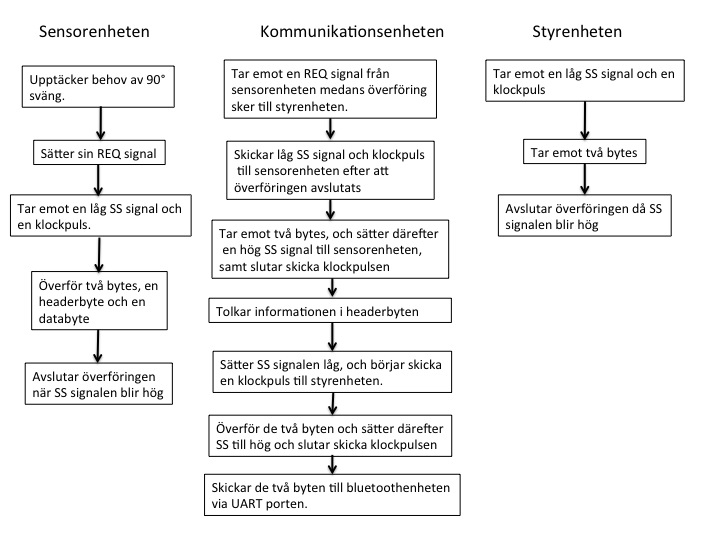
\includegraphics[angle=0,scale=0.5]{bilder/Schema_exempel.png}

\subsubsection{Övrigt om kommunikationsenheten}

Som nämnts tidigare kommer det vara kommunikationsenheten som sköter all kontakt mellan PCn och de olika enheterna. Det är på kommunikationsenheten som det kommer att finnas en brytare där användaren kan avgöra huruvida denna vill använda roboten i autonomt eller manuellt läge. Den största skillnaden i kommunikationsenhetens arbete mellan de två lägena är att sensorenheten inte kommer att användas i manuellt läge. Istället kommer alla styrkommandon att skickas till kommunikationsenheten via bluetooth. Kommunikationsenheten kommer också att vara den enhet som tillhandahåller en av- och påknapp för hela systemet.

Vid omställning till manuellt läge kommer det att överföras ett speciellt kommando till sensorenheten som beordrar denna att sluta avläsa sensorerna och begära dataöverföringar. Styrenheten kommer inte att behöva någon liknande kod då denna inte kommer att utföra någon reglering om den inte mottar någon reglerdata. Headerbyten kommer att användas för att instruera styrenheten om att mottagen information är specialkommandon som efterfrågar någon av typ av speciellt beteende.

